\documentclass[12, twoside]{report}
\usepackage[romanian]{babel}
\usepackage{ucs}
\usepackage[utf8x]{inputenc}
\usepackage[letterspace=100]{microtype}
\usepackage{graphicx}
\graphicspath{ {images/} }
\usepackage[a4paper, width=150mm, top=18.5mm, bottom=20mm, bindingoffset=12mm]{geometry}
\usepackage{titlesec}
\usepackage{indentfirst}
\usepackage{euscript}
\usepackage{enumitem}
\usepackage{fixltx2e}
\usepackage{chngcntr}
\usepackage{wrapfig}
\usepackage{underscore}
\usepackage{setspace}
\usepackage{parallel,enumitem}
\usepackage{minted}
\renewcommand\listingscaption{\textbf{Cod sursă}}
    
\usemintedstyle{colorful}
\usepackage[labelfont=bf]{caption}
\renewcommand{\figurename}{\textbf{Figura}}

\DeclareCaptionType{protocol}[Protocol][List of protocol]
\newenvironment{protenv}{}{\vspace{1.5em}}

\DeclareCaptionType{result}[Rezultat][List of result]
\newenvironment{rezenv}{}{\vspace{1.5em}}

% Table of contents customization

% link for table of contents
\usepackage[linktoc=all]{hyperref}
\hypersetup{ 
    colorlinks,
    citecolor=black,
    filecolor=black,
    linkcolor=black,
    urlcolor=black,
}

% dots filling
\usepackage{tocloft}
\renewcommand{\contentsname}{Cuprins}
\renewcommand{\cftpartleader}{\cftdotfill{.}}
\renewcommand{\cftchapleader}{\cftdotfill{.}}
\renewcommand{\cftsecleader}{\cftdotfill{.}}
\renewcommand{\cftsubsecleader}{\cftdotfill{.}}
\renewcommand{\cftdot}{.}

% space between lines in table of contents
\setlength{\cftbeforechapskip}{1.5ex}
\setlength{\cftbeforesecskip}{0.5ex}

% chapters font in table of contents
\renewcommand{\cftchapfont}{%
  \fontsize{11}{13}\usefont{OT1}{bch}{bc}{n}\selectfont
}

% reduce white space before and after the table of contents name
\setlength{\cftbeforetoctitleskip}{-1em}
\setlength\cftaftertoctitleskip{10pt}

% parag indentation
\setlength{\parindent}{7ex}

% chapters spacing
\titleformat{\chapter}[display]   
{\normalfont\huge\bfseries}{\chaptertitlename\ \thechapter}{20pt}{\Huge}   
\titlespacing*{\chapter}{0pt}{-25pt}{10pt}

% remove every Chapter i, i from 1 to nrOfChapters 
\titleformat{\chapter}[display]
  {\normalfont\bfseries}{}{0pt}{\huge}

% for using euler font with \mathcal{}
\DeclareMathAlphabet{\mathcal}{U}{eus}{m}{n}

\titlespacing*{\section}
{0pt}{0pt}{7pt}
\titlespacing*{\subsection}
{0pt}{0pt}{0pt}
\setlist[itemize,1]{leftmargin=\dimexpr 45pt}

\counterwithout{figure}{chapter}
\counterwithout{protocol}{chapter}
\counterwithout{result}{chapter}

% pentru cod
\usepackage{listings}

\lstset{
        basicstyle=\ttfamily\scriptsize,
       }
\renewcommand*{\lstlistingname}{Exemplo de código}

\title{
	{Security Protocols Checker}
}
\author{Ștefan Stan}
\date{April 2014}

\begin{document}

\begin{titlepage}
	\begin{center}
		\normalsize
		\hspace{1.9cm}		
		\textsf{UNIVERSITATEA ALEXANDRU IOAN CUZA IAŞI}
		\newline
		
		\vspace{0.1cm}
		\Large
		\textbf{FACULTATEA DE INFORMATICĂ}
		
		\vspace{2.75cm}
		\begin{figure}[h]
			\centering
    		
\includegraphics[scale=1.5]{fii}
		\end{figure}	

		\vspace{2.65cm}
		  
		{\fontsize{18}{21.6}\selectfont LUCRARE DE DISERTAȚIE\par}

		\vspace{1.2cm}
		\Huge
		\textbf{A study on point in time recovery on relational databases}		
		
		\vspace{1.2cm}		
		\Large
		\textbf{propusă de}		

		\vspace{1cm}
		\huge
		\textit{\textbf{Ștefan Stan}}		
		
		\vspace{1.1cm}
		{\fontsize{18}{21,6}\selectfont 		
		\textbf{Sesiunea: }
		\textit{Iulie, 2017}\par}		
		
		\vspace{2.2cm}
		{\fontsize{14}{18}\selectfont 		
		\textbf{Coordonator ştiinţific}\par}			
		
		\vspace{0.5cm}
		{\fontsize{18}{21,6}\selectfont 		
		\textbf{Lect. dr. Cristian Frăsinaru}\par}	
		
		\newpage
		
		\thispagestyle{empty} 
		\normalsize
		\hspace{1.9cm}		
		\textsf{UNIVERSITATEA ALEXANDRU IOAN CUZA IAŞI}
		\newline
		
		\vspace{0.1cm}
		\Large
		\textbf{FACULTATEA DE INFORMATICĂ}
		
		\vspace{7cm}

		\Huge
		\textbf{A study on point in time recovery on relational databases}	
		
		\vspace{1.2cm}			
		\vspace{0.2cm}
		\vspace{1.5cm}
		\huge
		\textit{\textbf{Ștefan Stan}}		
		
		\vspace{1.9cm}
		{\fontsize{18}{21,6}\selectfont 		
		\textbf{Sesiunea: }
		\textit{Iulie, 2017}\par}		
		
		\vspace{4.25cm}
		{\fontsize{14}{18}\selectfont 		
		\textbf{Coordonator ştiinţific}\par}			
		
		\vspace{0.5cm}
		{\fontsize{18}{21,6}\selectfont 		
		\textbf{Lect. dr. Cristian Frăsinaru}\par}			
		
		\vspace{0.5cm}
		{\fontsize{14}{18}\selectfont 		
		\textbf{Supervizor companie}\par}			
		
		\vspace{0.5cm}
		{\fontsize{18}{21,6}\selectfont 		
		\textbf{DevOps Engineer Gabi Ichim, TSS-Yonder}\par}			
		
		\normalsize
	\end{center}
\end{titlepage}
\newpage
\thispagestyle{empty}
\large
\textbf{DECLARAŢIE PRIVIND ORIGINALITATEA ŞI RESPECTAREA DREPTURILOR DE AUTOR}
\vspace{2.5cm}
\large
\par
Prin prezenta declar că lucrarea de desertație cu titlul "A study on point in time recovery on relational databases" este scrisă de mine şi nu a mai fost prezentată niciodată la o altă facultate sau instituţie de învăţământ superior din ţară sau străinătate. De asemenea, declar că toate sursele utilizate, inclusiv cele preluate de pe Internet, sunt indicate în lucrare, cu respectarea regulilor de evitare a plagiatului:
\\
\begin{itemize}
\item[--] toate fragmentele de text reproduse exact, chiar şi în traducere proprie din altă limbă, sunt scrise între ghilimele şi deţin referinţa precisă a sursei;
\item[--] reformularea în cuvinte proprii a textelor scrise de către alţi autori deţine referinţa precisă;
\item[--] codul sursă, imagini etc. preluate din proiecte open-source sau alte surse sunt utilizate cu respectarea drepturilor de autor şi deţin referinţe precise;
\item[--] rezumarea ideilor altor autori precizează referinţa precisă la textul original.
\end{itemize}
\vspace{5cm}
Iași,
\vspace{1cm}
\begin{flushright}
Absolvent \textit{Ștefan Stan}
\\
\vspace{0.6cm}
\rule{4.1cm}{0.4pt}

\end{flushright}

\newpage
\thispagestyle{empty}
\large
\begin{center}
\textbf{DECLARAŢIE DE CONSIMŢĂMÂNT}
\end{center}
\vspace{2.5cm}
\large
Prin prezenta declar că sunt de acord ca lucrarea de disertație cu titlul "A study on point in time recovery on relational databases", codul sursă al programelor şi celelalte conţinuturi (grafice, multimedia, date de test etc.) care însoţesc această lucrare să fie utilizate în cadrul Facultăţii de Informatică.
\\
De asemenea, sunt de acord ca Facultatea de Informatică de la Universitatea Alexandru Ioan Cuza Iaşi să utilizeze, modifice, reproducă şi să distribuie în scopuri necomerciale programele-calculator, format executabil şi sursă, realizate de mine în cadrul prezentei lucrări de disertație.
\\

\vspace{3.5cm}
\begin{flushleft}
Iași,
\end{flushleft}
\vspace{1cm}
\begin{flushright}
Absolvent \textit{Ștefan Stan}
\\
\vspace{0.6cm}
\rule{4.1cm}{0.4pt}

\end{flushright}

\newpage
% \thispagestyle{empty} supress the page number
% \textit{K}\rlap{\textsuperscript{\textit{e}}}\textsubscript{\textit{A}}
% \textit{\textit{K}}\rlap{\textsuperscript{\textit{d}}}\textsubscript{\textit{A}}
% \textit{\textit{K}}\textsubscript{\textit{AB}}

\tableofcontents

% for setting the spacing between lines at 1.5 default is  1.0
\renewcommand{\baselinestretch}{1.5} 

\renewcommand{\bibname}{Bibliografie}

\chapter*{Introducere}
\large
Avand în vedere contextul unui dezvoltator software, am observat în timpul experienței faptul ca pentru echipa efectivă de dezvoltare era destul de dificil de întreținut baza de date (incluzând deasemenea și operațiile de pornire/oprire, mai ales pentru juniori acest lucru putea pune probleme dacă baza de date se afla instalată pe o platforma UNIX). În cazul în care se dorea aplicarea unei strategii de point in time recovery pentru restabilirea bazei de date la o stare existentă la un moment dat, era nevoie de intervenția echipei de devOps, care se ocupa în mod expres de acest tip de operații, având cunoștințe avansate despre subiect.
\par
Astfel că, am observat necesitatea existenței unei aplicații care să ușureze operațiile asupra bazei de date, începand cu pornirea/oprirea/verificarea starii, până la întreaga operație de backup și point in time recovery(întoarcere la o stare existentă la un anumit moment dat). Această aplicație trebuia să fie intuitivă, ușor de folosit chiar și pentru cineva care nu avea cunoștințe de devOps, nefiind necesar accesul efectiv pe mașina de UNIX unde se afla clusterul de baze de date. Este de la sine înteles că aplicația ar trebui să detecteze toate bazele de date din clusterul de pe mașina pe care este încarcată și ar trebui să permită operațiile prezentate mai sus pentru fiecare instanță în parte.
\par
Impactele unei astfel de aplicații sunt atat de natură tehnică, le oferă dezvoltatorilor mai mult control asupra sistemului necesitând mai puține cunoștințe, precum și de business, nu mai trebuie angajată o echipă dedicată de devOps și prin urmare se reduc costurile.
\addcontentsline{toc}{chapter}{Introducere}

\chapter*{Contribuții}
În crearea aplicației am văzut o necesitate exitentă întâlnită la dezvoltatorii de software și am încercat să o rezolv. Procesul general de restabilire a unei baze de date este descris în \textit{Capitolul 1}.
\par
În \textit{Capitolul 2} se prezintă într-o manieră detaliată o metodă de organizare a sistemului de fișiere UNIX, urmând ca în \textit{Capitolul 3} să fie discutată arhitectura aleasă pentru dispunearea clusterului de baze de date pe sistemul de fișiere, precum și avantajele aduse de aceasta.
\par
Soluția software este trecută în revistă în \textit{Capitolul 4}. Astfel că, se prezintă arhitectura aplicației, urmată de fiecare componentă ce intră în alcătuirea ei. Tot în acest capitol este descrisă și setarea aplicației și a mediului de lucru în Amazon Web Services.
\par
\textit{Capitolul 6} oferă un ghid detaliat al aplicației, urmând ca în \textit{Capitolul 7} să fie discutate direcțiile de dezvoltare viitoare și idei de îmbunătățire ale platformei dezvoltate.
\addcontentsline{toc}{chapter}{Contribuții}

%{\setstretch{1.0}
\chapter{Point in time recovery}
"Point in time recovery" în contextul informaticii se referă la funcționalitatea unui sistem folosită de un administrator pentru a restabili sau recupera un set de date existent la un moment dat.
\par
PostgreSQL menține în fiecare moment un \textit{write ahead log} WAL în subdirectorul pg_xlog al directorului de bază unde avem clusterul de baze de date. Acest log reține fiecare schimbare facută în fișierele bazei de date. Există, în principiu, pentru momentele în care sistemul cedează. Dacă acest lucru se întampla, datele pot fi recuperate prin o executare a secventei instrucțiunilor din log de la momentul ultimei salvări până înainte de momentul critic. Totuși, existența acestui log face posibilă o a treia strategie de restaurare a bazei de date: putem combina un backup la nivel de sistem de fișiere a bazei de date cu un backup al fișierelor WAL. Dacă avem nevoie să recuperăm datele vom restaura backup făcut la nivel de sistem de fișiere și apoi vom executa o secvență de fișiere WAL pentru a aduce baza de date la o versiune stabilă. Această abordare este complexă și dificil de setat, dar are multe beneficii:
\begin{itemize}
\item Nu avem nevoie de o stare consistentă a backup la nivel de sistem de fișiere. Orice inconsistentă va fi remediată prin executarea secvenței de fișiere WAL (nu este cine știe ce diferit de ceea ce se întamplă în momentul în care sistemul își revine după ce a cedat). Astfel că, avem nevoie de un utilitar capabil să creeze salvări pe disc, tar zip etc.
\item De vreme ce putem folosi o secvență nedefinită de fișiere WAL, backup continuu se poate realiza pur și simplu arhivând fișierele WAL. Această tehnică este foarte folositoare în cazul bazelor de date mari, unde nu este avantajos să facem backup complet în mod frecvent.
\item Nu este necesar să executăm toată secvență de fișiere WAL. Putem să ne oprim la orice moment din timp în care baza de date era consistentă. Astfel că, această tehnică suportă \textit{point in time recovery}. Este posibil să restaurăm baza de date la orice moment existent dacă avem fișiere WAL.
\item Daca oferim încontinuu fișiere WAL unei mașini noi ce a fost încărcată de la aceeași salvare, putem avea un sistem aflat în hibernare pe care îl putem aduce în orice moment în funcțiune având setul de date aflat în producție.
\end{itemize}
Pentru a recupera date cu succes folosind strategia de arhivare continuuă este nevoie de o secvența continuuă de fișiere WAL arhivate ce există cel putin de la momentul în care am creat acel basebackup (o stare a bazei de date aflata pe disc, un checkpoint). Pentru a începe e nevoie să setam și să testăm procedura de salvare a fișierelor WAL, înainte de a face primul basebackup. In cele ce urmează vom discuta mecanismul de arhivare a fișierelor WAL.
\section{Setarea arhivarii fișierelor WAL}
Într-un mod abstract, un sistem PostgreSQL produce o secvență nedefinită de înregistrări WAL. Sistemul împarte această secvență în fișiere WAL, care sunt în mod normal de 16MB fiecare (deși dimensiunea segmentului poate fi alterată cand facem build la PostgreSQL). Fișierele segment au numele într-un format numeric care reflectă poziția lor în secvența abstractă WAL. Când nu folosim arhivarea fișierelor WAL sistemul creează cateva fișiere pe care le reciclează redenumindu-le pe cele vechi și marcându-le pentru ștergere.
\par
Când arhivăm datele WAL trebuie să prindem conținutul fiecarui segment de îndată ce devine complet și să salvăm datele undeva până ca segmentul devine reciclat și refolosit. În funcție de aplicație și harware folosit, pot exista mai mult moduri să "salvăm datele undeva": putem copia segmentul într-o locație pe un disc extern, le putem trimite în cloud pe un cont de Amazon S3, Google Drive... le putem trimite prin rețea oriunde etc. PostgreSQL încearca să nu facă supoziții despre modul de arhivare a datelor pentru a facilita munca administratorului. În schimb, PosgreSQL lasă administratorul să ofere o comandă shell ce se va executa pentru a copia orice segment complet oriunde trebuie să meargă. Această comandă poate fi la fel de simpla ca un \textbf{cp}, sau se poate invoca un script complex de linux.
\par 
Pentru a activa arhivarea WAL trebuie să se parcurga o serie de pași:
\begin{itemize}
\item să se seteze \textbf{wal_level} ca fiind \textbf{archive} sau mai mare. (wal_level determină câtă informație se scrie în fiecare WAL. Implicit e setat ca fiind \textbf{minimal}, ceea ce înseamnă că se scrie doar informația necesară pentru a se restaura dupa o problemă sau dupa o închidere imediată; \textbf{archive} adaugă informații necesare pentru arhivarea WAL; \textbf{hot_standby} adaugă informații necesare pentru a rula interogari în mod citire pe un server aflat in pauza; \textbf{logical} adaugă informații necesare pentru a suporta decodare logică)
\item să se specifice o comandă shell în parametrul \textbf{archive_command}. În comanda de arhivare, parametrul \%p este înlocuit cu calea către fișierul WAL, în timp ce parametrul \%f este înlocuit cu numele fișierului. Calea este relativă la fișierul curent (fișierul în care se află clusterul de baza de date). Cea mai simplă comandă este de genul:\\ \textbf{archive_command = 'test ! -f /mnt/server/archivedir/\%f \&\& cp \%p /mnt/server/archivedir/\%f'}\\
Comanda va copia segmentul WAL în directorul /mnt/server/archvedir.
\end{itemize}
După ce s-au înlocuit parametrii \%p si \%f cmd. ce fa fi exec. va arata astfel: \\
\textbf{test ! -f /mnt/server/archivedir/00000001000000A900000065 \&\& cp pg_xlog/00000001000000A900000065 /mnt/server/archivedir/00000001000000A900000065}\\
O comandă similară va fi executată pentru fiecare segment nou ce fa fi generat. Comanda de arhivare va fi executată sub acealași utitizator ca și serverul PostgreSQL. De vreme ce seria de fișiere WAL conține efectiv datele din baza de date, va fi nevoie ca datele arhivate să fie protejate de către accesul neautorizat. Putem să nu oferim drept de citire pentru grup și pentru ceilalți.
\par
Comanda de arhivare este important să returneze statusul 0. PostgreSQL, cand primește 0 va crede că fișierul a fost arhivat cu succes și îl va șterge/ marca pentru reciclare. Însă, un status diferit de 0 va spune PostgreSQL ca arhivarea a eșuat și acesta va păstra fișierul reîncercând ulterior.
\par
Comanda de arhivare ar trebui construită în așa fel încât să refuze să suprascrie fișiere pre-existente. Această funcționalitate este o metodă de siguranță prin care se asigură integritatea datelor în cazul unei erori a administratorului (trimite rezultatul de pe doua servere în același director).
\par
Este de preferat să se testeze comanda propusă pentru arhivare, astfel că aceasta sa nu suprascrie fișiere și să returneze status diferit de 0 cand se încearcă acest lucru. Comanda oferită ca exemplu mai sus asigură acest lucru prin pasul de testare inițial. Unix deține pe anumite platforme opțiuni precum \textbf{-i} ce pot fi folosite pentru a realiza același lucru, dar nu trebuie să ne bazam pe ele ci să verificăm codul returnat de fiecare dată.
\\
Aceste setări vor fi modificate în fișierul \textbf{postgresql.conf}
\vspace{4cm}
\section{Crearea unui basebackup}
Un basebackup este o salvare pe disc la un moment dat a bazei de date, de la care se va porni procesul de executare a fisierelor WAL.
\par 
Cel mai ușor mod de a crea un basebackup este folosirea utilitarei \textbf{pg_basebackup}. Se poate crea un basebackup fie ca și fișiere normale pe disc sau ca și arhivă(tar). Nu este neaparat nevoie să fim îngrijorați de timpul necesar crearii basebackup. Totuși, dacă serverul rulează cu opțiunea \textbf{full_page_writes} dezactivată s-ar putea observa o scadere în performantă, de vreme ce procedura de basebackup rulează automat cu opțiunea \textbf{full_page_writes} activată în mod forțat.
\par
Pentru a ne folosi de basebackup trebuie să reținem toate fișierele WAL din timpul creării basebackup și după. Pentru a ne ajuta în acest proces, procedura de basebackup creează un fișier backup_history ce este mutat imediat în locația fișierelor WAL. Fișierul este denumit după primul fișier care este necesar pentru recovery folosind acel basebackup. Odată ce procesul de basebackup s-a terminat cu succes nu mai este nevoie de fișierele WAL de dinainte de crearea basebackup, de vreme ce avem o stare stabilă a bazei de date la momentul creării basebackup, de la care se va porni un proces ulterior de executare a fișierelor WAL pentru revenirea în caz de dezastru a bazei de date.
\par 
De vreme ce trebuie să salvăm fișierele WAL arhivate până la momentul ultimului basebackup înseamnă că intervalul între care se creează basebackups trebuie ales în funcție de căt spațiu de stocare vrem să folosim pentru a salva fișierele WAL. De asemenea, este de considerat și timpul pe care vrem sa îl alocam unui eventual proces de restabilire a bazei de date. Dacă este necesar acest lucru va trebui să executam fiecare fișier WAL și ar putea dura destul de mult în caz că ultimul basebackup a fost facut acum mult timp.
\vspace{6cm}
\section{Restabilirea db. folosind Continuous Archive Backup}
Să presupunem că ce e mai rau s-a intamplat și e nevoie să restabilim baza de date. Procedura este urmatoarea:
\begin{enumerate}
\item
Se oprește serverul, dacă ruleaza.
\item
Se copie conținutul fișierul \textbf{pg_xlog} ce poate conține fișiere log cu motivele pentru care sistemul a ajuns într-o stare inconsistentă, precum și segmentele WAL nearhivate (ce nu au atins pragul necesar (implicit 16MB) pentru a fi arhivate)
\item
Se șterge orice fișier din locația clusterului de baze de date.
\item
Se copie datele ultimului basebackup în locația clusterului de baze de date. Trebuie verificate drepturile de acces la fișierele/directoarele copiate.
\item
Se șterge conținutul directorului pg_xlog copiat din basebackup, deoarece nu este de actualitate. Se copie fișierele din directorul pg_xlog salvat anterior.
\item
Se creează un fișier \textbf{recovery.conf}. De asemenea se va modifica și fișierul \textbf{pg_hba.conf} pentru a nu da voie utilizatorilor obișnuiți să se conecteze până când procesul de recuperare nu se termină.
\item
Se pornește server-ul. Acesta va intra automat în mod de recuperare și va începe să execute fișierele WAL, dacă există. Daca procesul eșuează din motive externe, se poate restarta serverul și va continua. În momentul în care procesul se termina se va redenumi fișierul \textbf{recovery.conf} în \textbf{recovery.done} pentru a preveni porniri ulterioare ale procesului de recuperare. Baza de date va funționa normal de acum.
\item 
Se inspectează baza de date pentru a se vedea dacă starea este una consistentă și dorită.
\end{enumerate}
Procesul se bazează pe setarea unui fișier de configurare \textbf{recovery.conf} ce specifică cum să se execute procesul și până când anume. Singurul lucru neaparat necesar în fișierul de restaurare este \textbf{recovery_command} care specifică ce comandă shell se va executa pentru a recupera fișierele WAL. Aceasta este construită precum \textbf{archive_command} prezentată anterior.\\
De exemplu: \textbf{restore_command = 'cp /mnt/server/archivedir/\%f \%p'}
%}

\chapter{Logical Volume Manager (LVM)}
În zilele de început ale serverelor Linux se făcea managementul spațiului de stocare prin crearea de partiții pe disc. Chiar dacă această abordare funcționează, ea prezintă anumite dezavantaje, iar cea mai importantă este aceeaa că discurile sunt inflexibile. Acesta este motivul pentru care a fost introdus Logical Volume Manager. Chiar dacă nu este posibil să schimbăm în mod dinamic marimea unei partiții care ramane fără spațiu, acest lucru este rezolvat lucrând cu LVM. LVM oferă multe avantaje ce vor fi prezentate în cele ce urmează.
\section{Arhitectura LVM}
În arhitectura LVM se pot distinge mai multe layere. Primul nivel lucrează direct cu componentele de stocare. Acesta este creat într-un mod abstract și poate folosi orice medii de stocare.
\par
Mediile de stocare trebuie marcate ca "physical volumes", ceea ce le face să poată fi folosite de către LVM. O componentă de stocare marcată ca "physical volume" poate fi adăugata unui "volume group", layer abstract peste toate mediile de stocare. Abstractizarea constă în faptul că acesta nu este ceva fix, poate fi redimensionat când este necesar, ceea ce face posibil să se adauge mai mult spațiu la nivelul "volume group" atunci când "logical volumes" ce fac parte din el rămân făra spațiu. Concret, dacă se rămâne fără spațiu pe un logical volume se ia din spațiul liber de la nivelul volume group-ului din care face parte. În cazul în care nici la acel nivel nu mai există spațiu liber se adaugă un disc nou în volume group. 
\par
Intuitiv, deasupra nivelului de volume groups se află logical volumes. Acestea nu actionează ca medii de stocare directe, ele își iau spațiul necesar din discurile aflate în volume group. Astfel că, un logical volume poate avea spațiul de stocare distribuit pe mai multe physical volumes (medii de stocare).
\section{Funcționalități LVM}
Există multe motive pentru care LVM este foarte util. Cel mai important motiv este acela că oferă flexibilitate pentru managementul spațiului de stocare. Partițiile nu mai sunt limitate de către spațiul de stocare al discurilor. Deasemenea, este posibil să se reducă mărimea unui logical volume, dar doar dacă sistemul de fișiere ce a fost creat suportă redimensionare. De exemplu, sistemul de fișiere Ext4 suportă redimensionare în timp ce XFS, care este sistemul de fișiere implicit de pe RHEL (Red Hat Enterprise Linux) nu suportă.
\par
Un alt motiv pentru care administratorii de sistem folosesc LVM este posibilitatea de a crea salvări. O salvare ține minte starea curentă a logical volume și poate fi folosită pentru a îl restaura dacă este nevoie.
\par
Al treilea avantaj important este acela că avem posibilitatea de a schimba ușor elementele hardware stricate. Dacă un hard disk se strică, datele pot fi mutate în cadrul volume group prin comanda pvmove și un nou harddisk se poate adauga dinamic fara a avea sistemul cazut.
\section{Crearea Logical Volumes}
Crearea Logical Volumes presupune crearea a trei layere în arhitectura LVM. În primul rând trebuie create PV(physical volumes), apoi urmează să se creeze VG(volume group) la care se adaugă physical volumes create anterior. În ultimul rând, trebuie create LV(logical volumes) pe care le vom folosi ca și "partiții" efective.
\par
Înainte de a folosi utilitarele LVM trebuie să marcăm partițiile hardware ca fiind de tipul LVM. Dacă se folosește utilitara fdisk împreună cu un disc de tip MBR, atunci partiția trebuie pusă de tipul 8e. Altfel, dacă se folosește gdisk împreună cu un disc de tip GUID, atunci partiția este de tip 8300.
\subsection{Pași pentru a crea un Physical Volume}
Avem nevoie de un harddisk care are spațiu liber (nepartiționat). Pentru scopul explicării se va folosi un disk /dev/vdb pentru a crea partiția. Fiecare disc are un nume diferit astfel că pașii vor trebui ajustați pentru fiecare disc.
\begin{itemize}
\item Se deschide un shell și se execută \textbf{fdisk /dev/vdb}
\item Se apasă \textbf{n} pentru a crea partiția. Se selectează \textbf{p} pentru a o marca partiție primară si se acceptă numerotarea implicită.
\item Se apasă \textbf{Enter} de două ori și astfel se creeză o partiție folosind tot spațiul de pe discul \textbf{/dev/vdb}
\item Fiind întors la prompter-ul fdisk, se apasă t pentru a schimba tipul partiției create. Fiind o singură partiție ce folosește întreg spatiul aceasta va fi selectată implicit, altfel ar putea întreba pentru care partiție să se schimbe tipul. 
\item Utilitara fdisk întreabă ce tip va avea partiția alesă. Scrie 8e. Apasă w pentru a scrie schimbările efectuate în acești pași. Dacă se primește un mesaj conform căruia tabela de partiții nu a putut fi actualizată trebuie dat un restart. 
\end{itemize}
Acum că partiția a fost creată trebuie marcată ca LVM physical volume. Pentru asta se va executa \textbf{pvcreate /dev/vdb1}. Ar trebui primit următorul mesaj: Physical volume “/dev/vbd1” successfully created. Pentru a verifica existența physical volume nou creat putem executa în shell comanda pvs ce listează physical volume existente.
\subsection{Pași pentru a crea un Volume Group}
Acum că am creat un physical volume trebuie să îl asignam unui volume group. Este posibil să adăugăm physical volumes la un volume group existent (a se citi manualul din linux pentru comanda \textbf{vgextend}), însă avem un volume group și vom adăuga un physical volume la el. Aceasta este procedura relativ ușoară, o singură comanda, vgcreate, ce primește numele noului volume group precum și physical volume ce va fi adăugat inițial. De exemplu: \textbf{vgcreate vgdata /dev/vdb1}.
\par Este complet la alegerea utilizatorului ce nume alege pentru volume groups. În acest exemplu am ales să încep numele cu vg, ceea ce le face ușor de găsit dacă vre-odată avem foarte multe. 
\par După ce s-a creat volume group putem executa comanda \textbf{vgs} pentru a lista volume groups existente.
\subsection{Pași pentru a crea Logical Volumes}
Acum că s-a creat un volume group putem începe să cream logical volumes. Procedura este un pic mai complicată decât crearea physical volumes sau volume groups, deoarece sunt mai multe alegeri ce trebuie făcute. Cand se creeaza un logical volumes trebuie specificate numele și mărimea.
\par
Mărimea logical volume poate fi specificată prin valoare absolută folosind opțiunea \textbf{-L}. De exemplu, folosind \textbf{-L 5G} se creează un logical volume cu mărimea de 5GB. O alternativă este să folosim opțiunea \textbf{- l} pentru a specifica o mărime relativă. De exemplu, se folosește \textbf{- l 50\% FREE} pentru a folosi jumătate din spațiul liber la nivelul volume group. Următorul argument este numele volume group la care va fi asignat logical volume nou creat și din care se va lua spațiu necesar. Un parametru opțional este \textbf{- n} ce specifică numele noului logical volume. De exemplu, comanda \textbf{lvcreate -n lvvol1 -L 100M vgdata} creează un logical volume cu numele lvvol folosind 100MB spațiu din volume group cu numele vgdata (creat anterior).
\subsection{Modificarea mărimii unui Logical Volume}
Motivul folosirii logical volumes în locul utilizării directe a unor discuri este acela că la nevoie putem foarte ușor să adăugam spațiu într-un logical volume, în timp ce dacă de exemplu, avem de adăugat în cazul discurilor trebuie să adăugam un alt disc mai mare și să copiem totul din discul inițial, moment în care sistemul trebuie să fie oprit. Daca de exemplu avem un folder /tenant1 în care ținem datele din baza de date pentru un client. Să ne imaginăm că acesta trimite la un disc fizic de 100GB. Pentru a putea să oferim mai mult spațiu în acest director va fi nevoie să oprim baza de date, să mutăm toate datele pe un alt disc de 200GB de ex și apoi să repornim sistemul. În cazul în care /tenant1 este un director la care a fost montat un logical volume putem folosi urmatoare procedura pentru a mări spațiul fără a opri sistemul:
\begin{itemize}
\item Verificăm că în volume group din care face parte logical volume ce va fi extins se află spațiu liber. Dacă nu există spațiu liber, adaugă un nou physical volume.
\item Executăm comanda \textbf{vgextend} pentru a extinde spațiul din logical volume.
\end{itemize}
Putem utiliza comanda \textbf{lvs} ce listează date despre logical volumes existente pentru a vedea spațiul liber al logical volume. Pentru detalii despre comanda \textbf{vgextend} sa se execute comanda \textbf{man vgextend} ce afișeaza manualul din Linux.
\newpage
\section{Convenția de numire a LVM}
Din acest moment putem începe să folosim logical volume nou creat. Pentru a face asta trebuie să stim cum să ne adresăm acestuia. Entitățile LVM pot fi adresate în moduri multiple. Cea mai simplă metodă este să adresăm un logical volume precum: /dev/vgname/lvname. Astfel că, dacă am creat un logical volume cu numele lvdata, ce își ia spațiu dintrun volume group cu numele vgdata, calea entității va fi /dev/vgdata/lvdata.
\par
Device mapper poartă un rol important în denumirea LVM logical volumes. Device mapper (abreviat dm) este o interfața generică folosită de kernelul Linux pentru a adresa device de stocare. Device mapper este folosit de către multiple sisteme: LVM volumes, dar și de software RAID etc. Aceste device sunt create în două locații: device numerotate în secvență plasate în directorul /dev, precum /dev/dm-0, /dev/dm-1 și așa mai departe. Deoarece aceste denumiri nu oferă nicio informație despre deviceuri ci confuzează, se folosesc scurtături create în directorul /dev/mapper. Acestea folosesc șablonul vgname-lvname pentru nume. Astfel că, dacă avem device /dev/vgdata/lvdata putem să ne adresăm folosind și /dev/mapper/vgdata-lvdata. Când lucrăm cum LVM logical volumes putem folosi oricare din aceste tipuri de adresare.

\chapter{Database Point in time recovery Manager}
Din punctul de vedere al unui dezvoltator software am observat în timpul experienței faptul că pentru echipa efectivă de dezvoltare era destul de dificil de întretinut baza de date (mă refer chiar și la pornit/oprit, mai ales pentru juniori acest lucru putea pune probleme dacă baza de date se afla instalată pe o platforma UNIX). În cazul în care se dorea aplicarea unei strategii de point in time recovery pentru restabilirea bazei de date la o stare existentă la un moment dat, era nevoie de intervenția echipei de devOps, ceea ce se factură diferit la client, prin urmare trebuia convins în prealabil Product Owner-ul de necesitatea acelei intervenții si planificat totul.
\par
Astfel că, am observat necesitatea existenței unei aplicații care să ușureze operațiile asupra bazei de date, începând cu pornirea/oprirea/verificarea statusului până la întreaga operație de backup și point in time recovery(întoarcere la o stare existentă la un anumit moment dat). Aceasta aplicație trebuia să fie intuitivă, ușor de folosit chiar și pentru cineva care nu avea cunoștinte de devOps, nefiind necesar accesul efectiv pe mașina de UNIX unde se afla clusterul de baze de date. Este de la sine înteles că aplicația ar trebui să detecteze toate bazele de date din clusterul de pe mașina pe care este încărcată și ar trebui să permită operațiile prezentate mai sus pentru fiecare instanță în parte.
\par
Am propus o soluție pentru bazele de date PostgreSQL folosite pe platforme UNIX (la momentul de față). Pentru a prezenta soluția software am avut nevoie de un mediu UNIX pe care să ruleze un numar de instanțe PostgreSQL. Am ales o mașină CentOS, instanța EC2 oferită de Amazon. Sistemul de fișiere a fost organizat folosind LVM (logical volume manager) dupa cum urmeaza:
\begin{itemize}
\item am cerut 3 discuri de câte 50GiB, Amazon EBS;
\item am creat cate un physical volume din fiecare din cele 3 discuri;
\item am creat un volume group și le-am adăugat acestuia;
\item am creat 6 logical volumes, 3 seturi de cate 2 logical volumes; un logical volume de 20GiB pentru datele din db și un logical volume de 10GiB pentru stocarea fișierelor WAL.
\end{itemize}
Au mai ramas 60GiB nealocați, aceștia putând fi folosiți ulterior. Dacă se observă că un client are nevoie de mai mult spațiu i se pot extinde logical volumes folosind din spațiul nealocat, acesta fiind marele avantaj al LVM. Bazele de date nu vor fi întrerupte cât timp se face extinderea logical volumes.
\par
Am setat astfel sistemul de fișiere pentru 3 instanțe diferite de baze de date PostgreSQL denumite lv-pgdata-1, lv-pgdata-2 si lv-pgdata-3. În \textit{Figura 1} este prezentată diagrama sistemului de fișiere.
\begin{figure}[h]
	\centering
	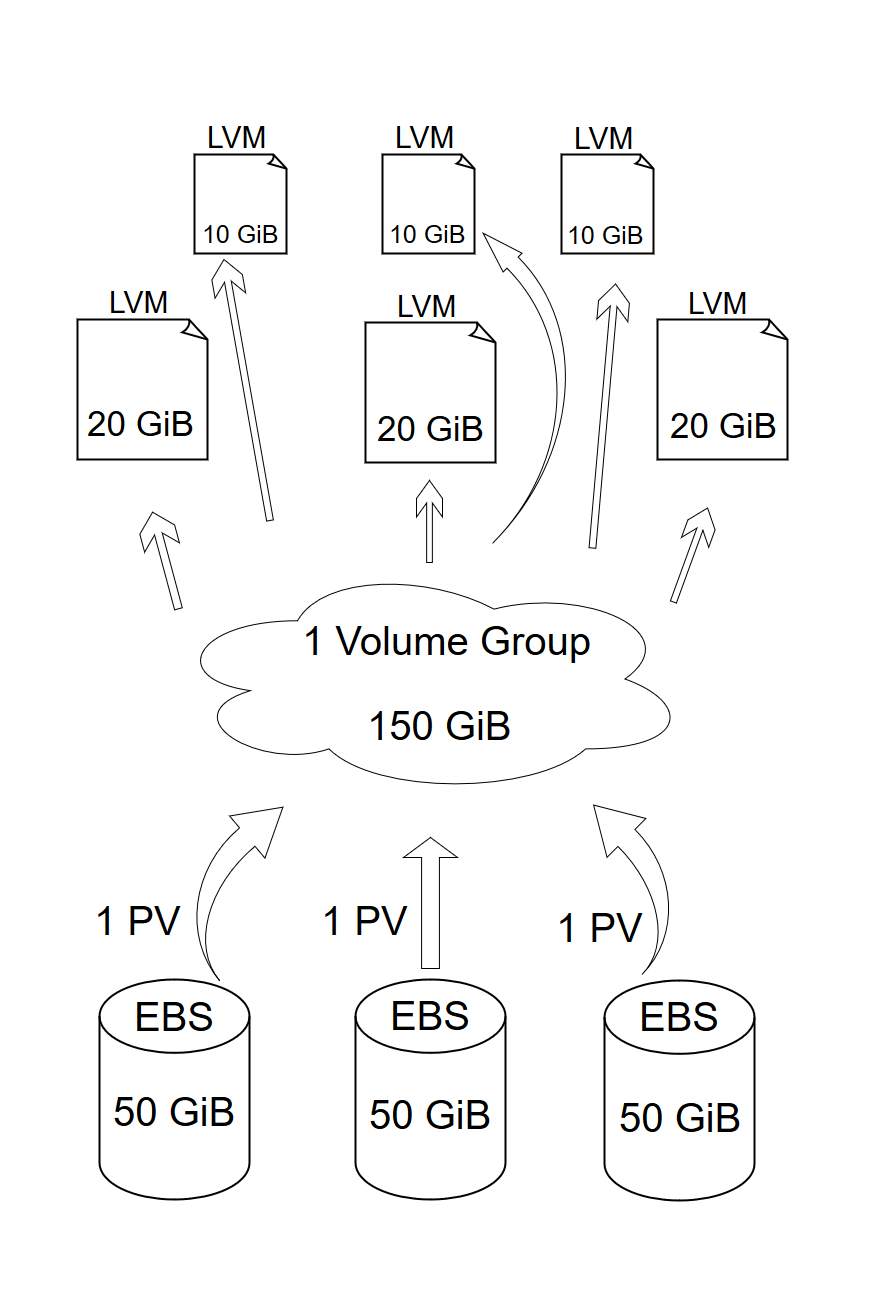
\includegraphics[scale=0.555]{LVM}
    \caption{Diagrama sistemului de fisiere}
    \label{fig:diagSistFiles}
\end{figure}

\chapter{DevOps as a Service}
In cele ce urmeaza voi prezenta solutia software propusa pentru managementul bazelor de date in maniera descrisa anterior. Voi trece in revista arhitectura software, urmand apoi sa explic fiecare din componentele aplicatiei, precum si modul de interactionare a acestora.
\\

\section{Arhitectura Sistemului Software}
Sistemul este impartit in 3 componente importante:
\begin{itemize}
\item Scripturi UNIX ce interactioneaza cu instantele de baze de date;
\item RESTful API folosit pentru a expune functionalitatea oferita de scripturi prin intermediul protocolului HTTP;
\item Aplicatie Web ce comunica prin intermediul protocolului HTTP cu API-ul RESTful expus.
\end{itemize}
In \textit{Figura 2} este prezentata diagrama arhitecturii software.
\begin{figure}[h]
	\centering
	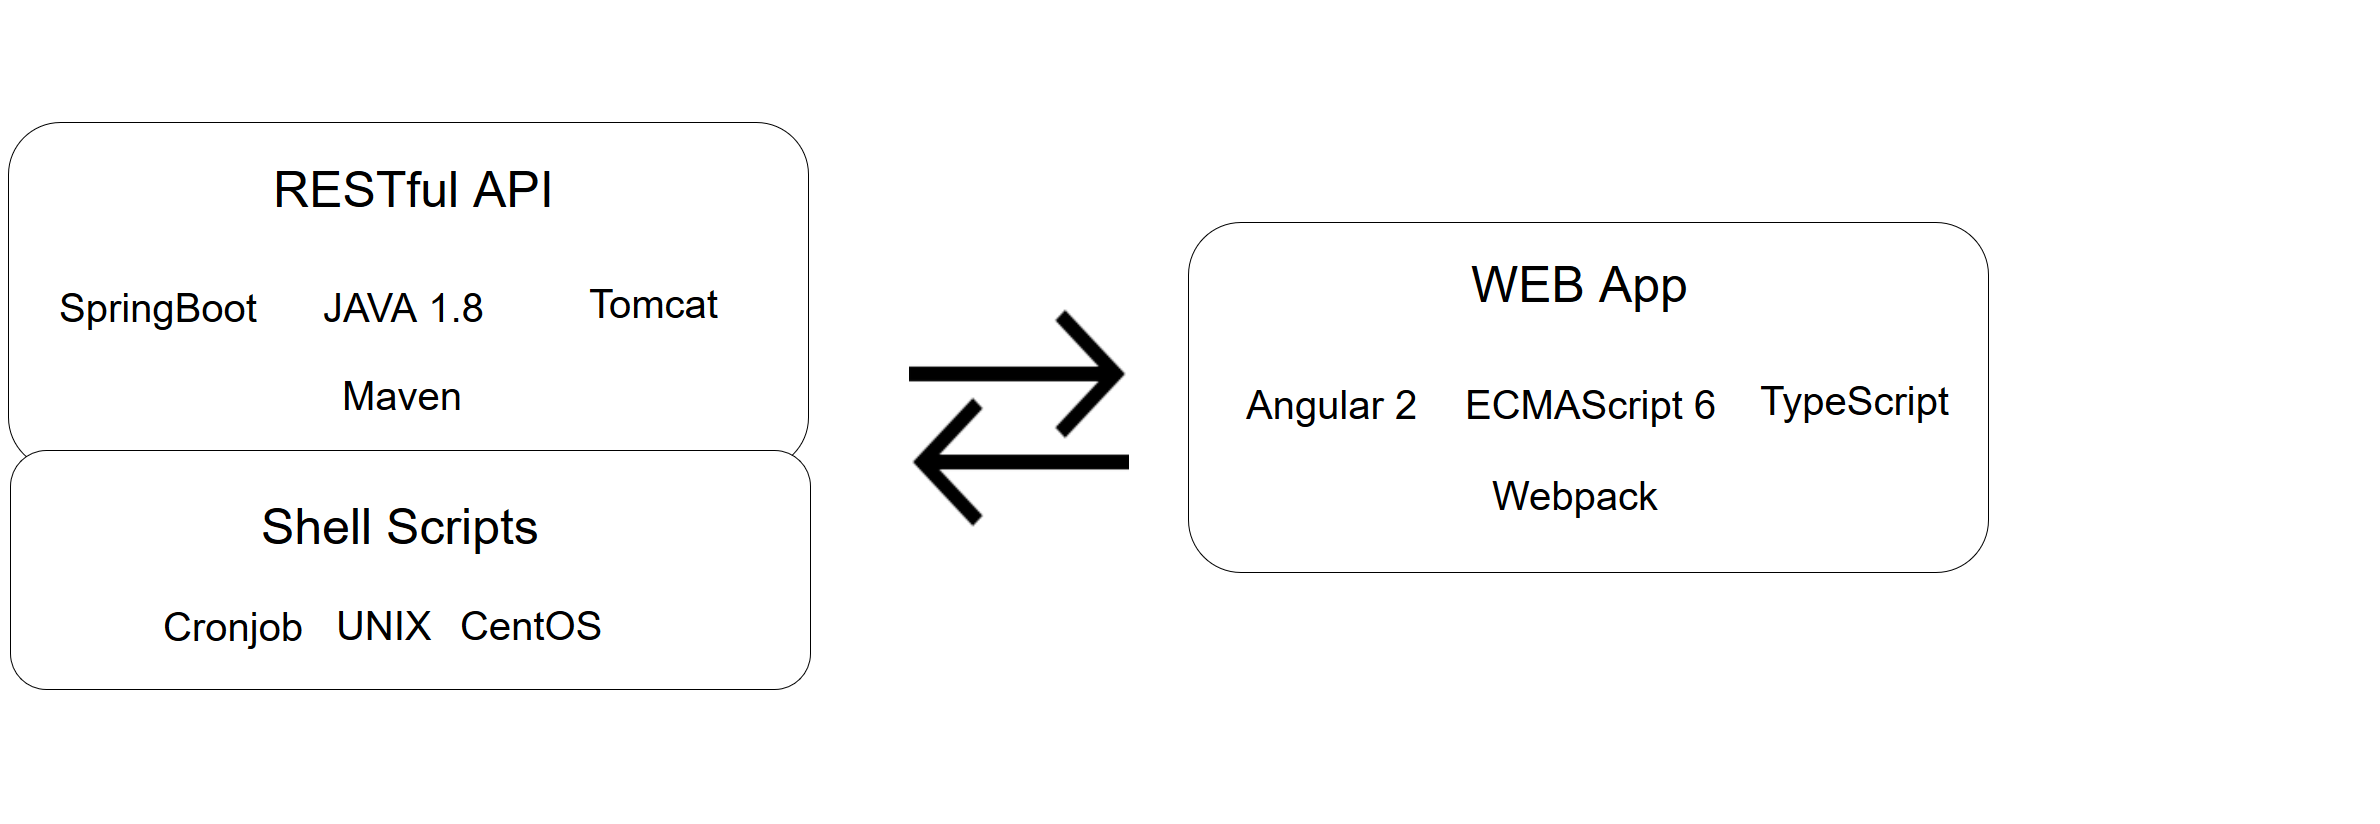
\includegraphics[scale=0.30]{LayeredArchLandscape}
    \caption{Diagrama arhitecturii software}
    \label{fig:LayeredArchPortrait}
\end{figure}
\newpage
\section{Scripturile UNIX}
Functionalitatea de baza a aplicatiei consta in interactionarea cu instantele de baze de date. Pentru asta am facut 3 scripturi ce au urmatoarele responsabilitati:
\begin{enumerate}
\item \textbf{pg-script.sh} pentru interactionarea cu instantele (pornire, oprire, interogare status);
\\
\begin{listing}[ht]
\inputminted[
frame=lines,
framesep=2mm,
baselinestretch=0.9,
fontsize=\footnotesize,
fontfamily=courier,
linenos
]{bash}{sourceCode/pg-script.sh}
\caption{\texttt{pg-script.sh}}
\label{cod:pgScript} 
\end{listing}
\item \textbf{basebackup.sh} pentru crearea de basebackup a unei instante (checkpoint de la care sa se poate incepe procesul de restaurare);
\\
\begin{listing}[ht]
\inputminted[
frame=lines,
framesep=2mm,
baselinestretch=0.9,
fontsize=\footnotesize,
fontfamily=courier,
linenos
]{bash}{sourceCode/basebackup.sh}
\caption{\texttt{basebackup.sh}}
\label{cod:basebackup} 
\end{listing}
\item \textbf{recovery.sh} pentru initierea procesului de restaurare a bazei de date
\\
\begin{listing}[ht]
\inputminted[
frame=lines,
framesep=2mm,
baselinestretch=0.9,
fontsize=\footnotesize,
fontfamily=courier,
linenos
]{bash}{sourceCode/recovery.sh}
\caption{\texttt{recovery.sh}}
\label{cod:recovery} 
\end{listing}
\end{enumerate}\
\par
Toate cele trei scripturi au fost gandite cu scopul de a se crea symbolic links (scurtaturi) catre ele. Acestea vor avea numele instantei bazei de date, iar scriptul principal foloseste numele fisierului scurtatura pentru a accesa datele instantei respective. Scopul este acela de a crea un singur set de scripturi, iar daca avem n instante de baza de date doar creem symbolic links catre scripturi, fiecare cu numele instante de baza de date respective.
\newpage
\section{Server-ul: RESTful API}
Pentru partea de server (backend) a fost aleasa solutia crearii unui RESTful API cu scopul de a se expune functionalitatea oferita de catre scripturile bash prezentate anterior. Am utilizat Java Enterprise Edition, framework-ul Spring, ce facilteaza crearea unui API prin intermediul librariilor SpringWeb.
\par
Un alt motiv pentru care am ales Spring a fost suportul oferit pentru a injecta dependinte urmand sablonul de proiectare Dependency Injection. Astfel, am decuplat controller-ul REST ce primeste cererea web de catre serviciul care o executa. Se poate injecta orice implementare de serviciu in controller, iar codul acestuia nu trebuie schimbat. Versiunea de Java utilizata este 1.8.
\begin{listing}[ht]
\inputminted[
frame=lines,
framesep=2mm,
baselinestretch=0.9,
fontsize=\footnotesize,
fontfamily=courier,
linenos
]{java}{sourceCode/DatabaseManagementAPI.java}
\caption{\texttt{DatabaseManagementAPI.java}}
\label{cod:DatabaseManagementAPI} 
\end{listing}
\newpage
Pentru managementul dependintelor si crearea artefactului s-a folosit Maven. Se ofera ca si exemplu fisierul \textbf{pom.xml}:
\begin{listing}[ht]
\inputminted[
frame=lines,
framesep=2mm,
baselinestretch=0.9,
fontsize=\footnotesize,
fontfamily=courier,
linenos
]{xml}{sourceCode/pom.xml}
\caption{\texttt{pom.xml}}
\label{cod:pom} 
\end{listing}

\newpage
\section{Interfata grafica cu utilizatorul}
Scopul proiectului este crearea unei aplicatii care sa faciliteze manipularea serverelor de baze de date PostgreSQL de catre dezvoltatori care nu trebuie sa aiba acces la masinile pe care se afla bazele de date/ cunostinte de UNIX. In acest sens, avand deja server-ul de Java care expune prin servicii Web functionalitatile respective, trebuie apelate si oferite intr-o maniera cat mai intuitiva. 
\par
Ca si framework am folosit Angular 2, limbajul de programare fiind Javascript, standardul ECMAScript6, impreuna cu TypeScript. Angular 2 are urmatoarele avantaje:
\begin{itemize}
\item este un framework open-source JavaScript construit și întreținut de Google, ceea ce usurează dezvoltarea aplicațiilor web.
\item standardizează aplicațiile la nivel de client (browser), oferind o structură robustă și ușor de implementat în dezvoltarea site-urilor.
\item este alegerea potrivită pentru orice aplicație web, în special dacă se preferă efectele vizuale spectaculoase. Rezultatul este un site fluid și rapid. Acesta este motivul pentru care se pretează SPA-urilor (Single Page Application) și aplicațiilor web destinate dispozitivelor mobile.
\item se integrează ușor cu Bootstrap, permite crearea de aplicații responsive care pot fi accesate atât din browserul calculatorului cât și de pe dispozitivele mobile. Astfel, este ușor să creezi o singură aplicație web care să se vadă perfect pe orice dispozitiv de pe care este accesată – PC, tabletă, telefon, plasmă.
\end{itemize}
\par Ca si manager de pachete am utilizat \textbf{npm} de la NodeJS.
\newpage
\section{Setarea aplicatiei in Amazon Web Services}
Avand ca si obiectiv crearea unui mediu cat mai apropiat de cel aflat pe masinile din productie, am inchiriat un server EC2 de la Amazon.
\par
Sistemul de fisiere a fost stabilit conform descrierii din Capitolul 2. Am inchiriat 3 discuri EBS(Elastic Block Storage) pe care le-am configurat precum a fost prezentat, pentru a seta 3 instante de baza de date.
\par 
Odata ce sistemul de fisiere a fost configurat, am creat scripturile ce vor interactiona cu bazele de date. Urmatorul pas a fost pornirea celor doua servere (backend si frontend). In timpul acestui proces a fost necesara configurarea unui rol de securitate oferit masinii de calcul EC2, pentru a permite traficul pe portul 3001 utilizat de aplicatia frontend.

\chapter{Ghid de utilizare a aplicaţiei}
Soluția propusă pentru a rezolva problema prezentată în capitolele procedente este o aplicație web folosită pentru managementul bazelor de date.
\par 
Aceasta oferă funcționalitățile de vizualizare a stării instanțelor de baze de date prin apăsarea butonului de "Refresh". Pentru a restaura starea bazei de date este necesară crearea unui checkpoint, iar pentru aceasta se apasă butonul "Create basebackup".
\par
Odată existent un checkpoint, se poate restaura baza de date respectivă prin alegerea unei date/ore folosind componenta vizuală de tip calendar, urmând să se apese butonul "Revert".

\chapter{Direcţii de dezvoltare viitoare}
Aplicatia propusa pentru a rezolva necesitatea restaurarii bazelor de date la anumite momente in timp poate fi folosita doar pentru baza de date PostgreSQL. 
\par
Astfel ca, o prima idee de dezvolatare viitoare ar fi investigarea suportului oferit alte tipuri de baze de date Oracle, MySql etc. urmand ca apoi sa creez un design abstract in ceea ce priveste baza de date si care sa fie integrat cu solutia existenta oferita pentru PostgreSQL.
\par
Cat despre interactiunea cu ultilizatorul, am folosit ultimele tehnologii actuale Angular 2, EcmaScript 6 etc. insa din punct de vedere al design, ar putea fi imbunatatit in ceea ce priveste html si css existent.

\chapter*{Concluzii}
Am creat o aplicație pornind de la necesitatea prezentată în capitolul \textit{Introducere}. Scopul acesteia este de a oferi o metodă facila de a restaura o baza de date la un moment de timp oferit de către utilizator. Acesta nu necesită cunoștințe de baze de date, sau de devOps (nu e nevoie să interacționeze cu scripturi de UNIX).
\par
Pentru a realiza cele menționate anterior am studiat modalitatea bazei de date PostgreSQL de management intern a transacțiilor și am utilizat-o întro manieră ce îmi permite restaurarea bazei de date la un moment în timp cu o granularitate fină, la secundă.
\par
De asemenea, am studiat modalitatea sistemului de operare UNIX ce permite creare de partiții virtuale ce pot fi oricând modificate în ceea ce privește mărimea fără a închide baza de date. Am combinat aceasta funcționaliate a sistemului de operare împreuna cu soluția propusă, pentru a realiza cele prezentate cu un timp minim de inaccesibilitate a bazei de date. \textit{Capitolul 3} prezinta în detaliu aceste aspecte.
\par
Am propus o arhitectură a sistemului de fișiere bazat pe studiul prezentat anterior și am utilizat-o în implementarea propriu-zisa. Cât despre aceasta, am folosit serviciile Amazon Cloud (EC2, EBS) pentru a face deploy soluției (scripturi ce interacționează cu baza de date, aplicație backend și aplicație frontend).
\par
In opinia mea, prin studiul realizat și prin intermediul soluției propuse am reușit să realizez ce mi-am propus și am oferit o modalitate de management a bazelor de date și de restaurare a acestora la starea existentă un moment de timp. Prin urmare am realizat o aplicație usor de utilizat de catre persoane ce nu au cunoștințe de baze de date, sistem de operare UNIX.
\addcontentsline{toc}{chapter}{Concluzii}

%\bibliography{myBib}

\begin{thebibliography}{10}

\bibitem{RHEL}
\newblock Sander van Vugt,
\newblock Red Hat® RHCSA™/RHCE® 7 Cert Guide: Red Hat Enterprise Linux 7 (EX200 and EX300)

\bibitem{GOF}
E.~Gamma, R.~Helm, R.~Johnson, and J.~Vlissides.
\newblock {\em Design Patterns: Elements of Reusable Object-Oriented Software}.
\newblock Addison-Wesley, 2005.

\bibitem{PITR}
Postgres Documentation
\par
\newblock https://www.postgresql.org/docs/9.5/static/continuous-archiving.html

\bibitem{SPRING}
\newblock {Craig Walls},
\newblock Spring in Action, Third Edition

\bibitem{MVC}
Martin Fowler.
\newblock {\em GUI Architectures}.
\newblock 18 July 2006.

\end{thebibliography}

\addcontentsline{toc}{chapter}{Bibliografie}

\end{document}